
\section{Architecture} \label{sec:Architecture}
This section starts with the architecture of a scalable prediction system in
\autoref{subsec:prediction_system}, and then we discuss the feasibility and
advantages of inline method to expose KPIs in \autoref{subsec:exposingAPI}.
\subsection{Scalable Prediction System} \label{subsec:prediction_system} We
propose a two-tiered system to implement an KPI computing system. We have a
proxy sitting at data plane; and local and central bandwidth estimator at control
plane. The local bandwidth estimator communicates with eNodeBs and it takes
channel quality, number of active users, cell load and users' queue size etc.
information as inputs and compute the available bandwidth for each user. A local
bandwidth estimator is logically distributed in the RAN and thus can be easily
scale-out. Meanwhile the central bandwidth estimator sits in the core network
and it summarizes local BW estimation and MME Mobility information to compute
the final bandwidth prediction for a user. In most cases one local estimation is
enough, however in cases like handoff we need choose among several local
estimations. Central estimators can be
scale-out with MMEs. Our architecture is generic and able to integrate into both
3G and 4G networks. 

Once the computation work is finished, the central estimator sends the
information to the proxy. 
 
\begin{figure}[tb]\label{fig:Architecture}
 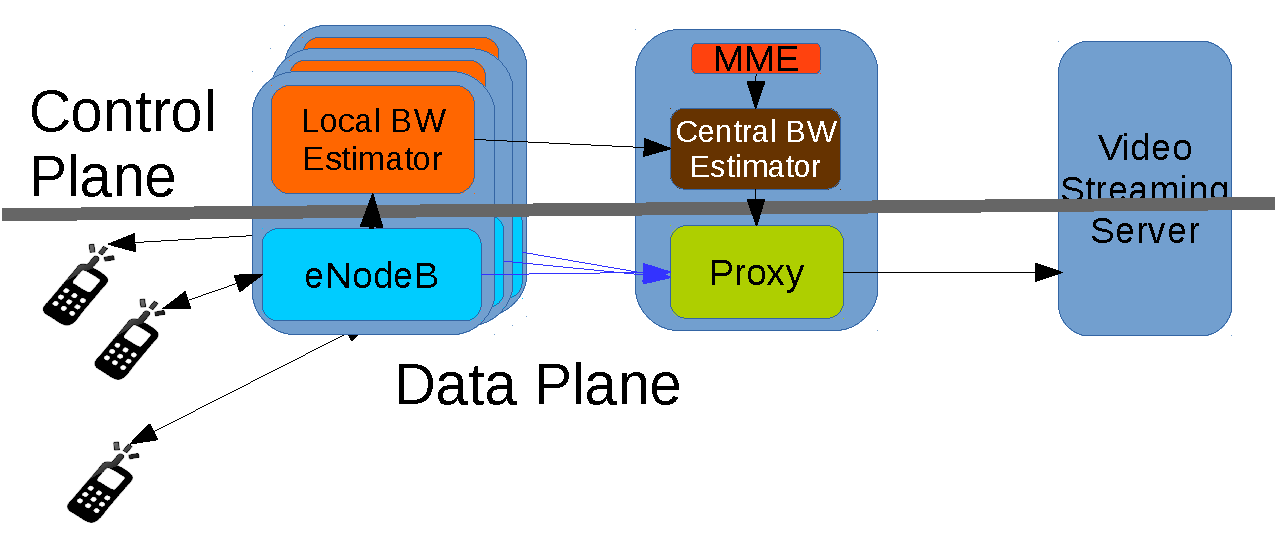
\includegraphics[width=\linewidth]{pictures/architecture2.pdf}
 \caption{Architecture for KPI Computing And Feedback}
\end{figure}


\subsection{KPI Exposure}\label{subsec:exposingAPI}
Current cellular networks already deploy proxies in the core network for
pacing purpose\cite{UntoldMiddleBoxStory}. It splits the TCP connection into two: server$\leftrightarrow
$proxy and proxy$\leftrightarrow $client. We can utilize the proxy for KPI
exposure. \emph{Sending to the server or the client?} We argue that exposing the
KPIs to the server causes less security concerns and network congestion. It also reduces the traffic in
the core network as sending to the client requires central estimator to send
back to local ones again. The downstream link carries majority of the traffic, upstream only has a small fraction of the traffic for feedback data. 
However since we let the server decide and the server in practice
may send back to the client's video play application. 

In terms of encoding the KPIs, there are several options: (i) in TCP; (ii) in
HTTP; and (iii) through a new connection. Inline methods have advantages over
new connection. First new connection method doubles the connections between the
server and the proxy. Second in practice CDNs are using public IPs, and the
video streaming connection and metric exposure connection may be directed to different private servers in CDN
load balancer. Inline methods both have some disadvantages. 
If we encode it into TCP option field, any middleboxes on the Internet may modify/drop the option field. 
The HTTP header may not be accessible since many streaming
services are using secure encrypted HTTP. Modifying HTTP header also requires DPI, which has a higher overhead than changing TCP.
\begin{figure}[t]\label{fig:Datagram}
 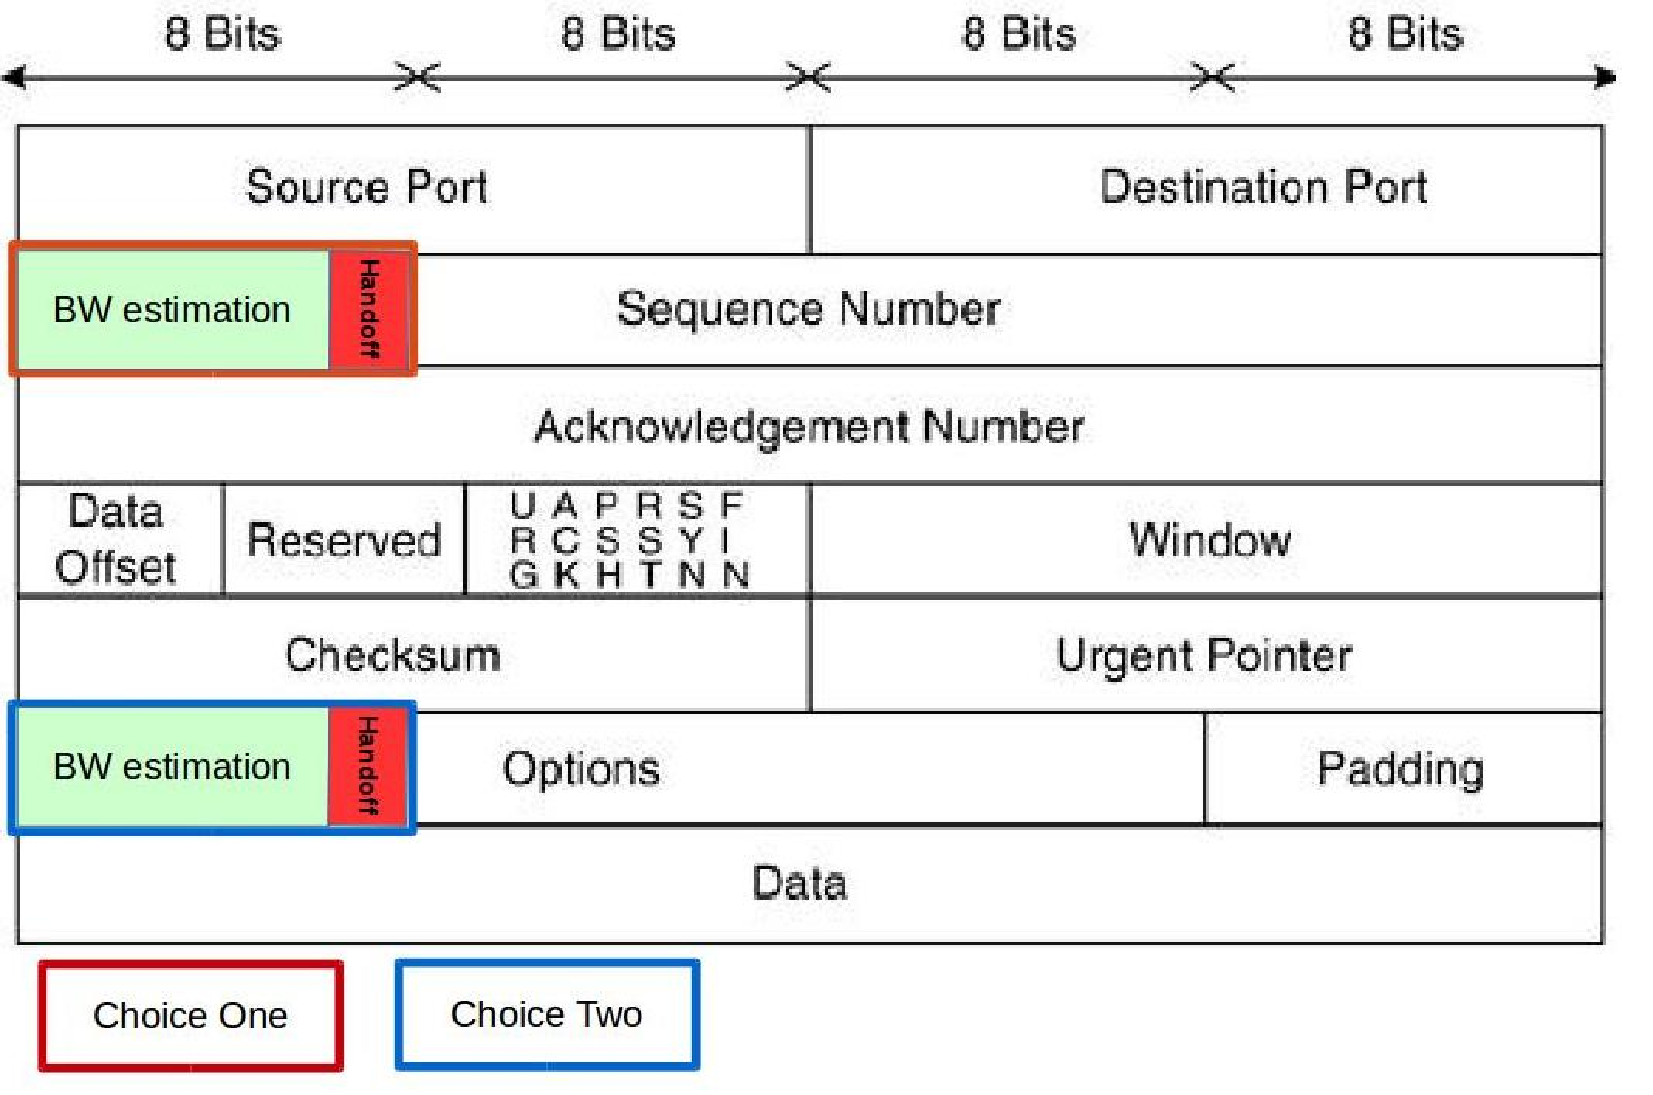
\includegraphics[width=\linewidth]{pictures/datagram.pdf}
 \caption{Datagram for exposing KPIs, it can be encoded in either option field or sequence number}
\end{figure}

One alternative approach is to encode in sequence number, if both content providers and cellular service providers are willing to collaborate. Since sequence number filed has 32 bits, we can reserve 8 bits for KPI exposure. In particular, we can use 7 bits for a floating number and 1 bit for handoff. Seven bits can be divided into integer and fractional parts, 3 bits for integer and 4 bits for fractional, it has a precision of 0.063 Mbps, or 63 Kbps and a maximum value of 8.94 Mbps, which is sufficient for today's video streaming bit rate selection where the range is between 0.2 to 4 Mbps.
At the same time it can still support 16 million packets before wrapping around. The bandwidth estimation is close to random so it holds the random feature of initial sequence number.

\xin{Would any middleboxes on the
Internet (between the proxy and the server) modify/drop the TCP option fields?}

\xin{Can we say a bit more about API here? What do the APIs look like? Give an
example and show how it is encoded in TCP option field.}

<emir>

In this section, we briefly describe the proposed architecture for realizing OpenCell concept. While alternative architectures are certainly possible, we aim for easy integration with the client-driven adaptation process in the state-of-the-art DASH systems. Hence, the exposed information or network state (e.g. predicted throughput) is made available to the client (video app), which can use it as a part of its adaptation logic, and/or share with the content server if desired.

The process of generating and exposing the information starts at the base station (eNodeB), where cell load, signal statistics and user throughput are collected. Based on collected data, predicted throughput is generated for all users and reported to the OpenCell server once per reporting interval. OpenCell server stores this information, which can be queried by user clients. Clients are typically HTTP-based and OpenCell server can use a simple HTTP-based API. Depending on requirements, clients can query the network state for the current or even past reporting periods. 

OpenCell servers can further process information received by base stations, e.g. to produce aggregated or long-term predictions. If base stations report every 500 ms, OpenCell servers may construct a prediction for 2, 5, or any number of seconds. This may depend on frequency the clients may query the OpenCell servers. 

In an application- or service-specific scenario, only certain apps or services are allowed to query OpenCell servers, enforcement of which is out of scope of this paper. However, it is possible to envision that all mobile clients could potentially have access. In a client-oriented architecture like ours, OpenCell servers are located inside the cellular core network and queried by video apps via HTTP. The prediction delivered by the OpenCell server will be valid for the next several seconds, typically on the order of video chunk duration. Each response may include information on how often clients may issue queries and for how long the returned prediction is valid.

We estimate that the proposed architecture can scale up to the requirements of today's video streaming services. 
(Add actual numbers)











